\documentclass[11pt]{article}

%aliases
\def\hf{\frac12}

%\usepackage{abbrevs}
\usepackage{natbib}
\usepackage{hyperref}
\usepackage{graphicx}     % could insert ``draft'' between []
\usepackage{caption}
\usepackage{amsmath,amsfonts}
\usepackage{enumitem}
%\usepackage{subcaption}
\pagestyle{empty}

\setlength{\oddsidemargin}{0pt} % there is 1 inch before the
                                % side margin in ``article'' class
\setlength{\textwidth}{6.5in}

\setlength{\voffset}{0pt}
%\setlength{\topmargin}{-36pt}     % there is 1 inch before the
\setlength{\topmargin}{-0.75in}     % there is 1 inch before the
                                % top margin in ``article'' class and
                                % then room for header, etc.
\setlength{\textheight}{9.5in}
%%%%%%%%%%%

\begin{document}
{\centering{\bf\Large HERA : Antenna Design Discussion} \\}
{
\centering{\bf\large Hydrogen Epoch of Reionization Array \\}
}
\vspace*{0.5cm}

\section{Cost Vs. Sensitivity}
    We weigh the cost and sensitivity benefits of the HERA antenna and array.
In order to accomplish this we define our figure of merit as the inverse of the
Cost (C) times the sensitivity ($\Delta_{N}^{2}$):
\begin{equation}
\label{eqn:fom}
    F.O.M = [C \times \Delta_{N}^{2}]^{-1}.
\end{equation}
The goal is to maximize the figure of merit.

Our sensitivity is proportional to $k^{3}$, $N^{-1}$, $u^{\frac{1}{2}}$, and
$\Omega^{\frac{5}{2}}$. $N$ is the number of antennas, $u$ is the baseline
length, and $\Omega$ is the beam size. Therefore, 
the sensitivity goes as
\begin{equation}
\begin{split}
    \Delta_{N}^{2} &\propto k^{3}N^{-1}u^{\frac{1}{2}} \Omega^{\frac{5}{2}} \\
    \Rightarrow \Delta_{N}^{2} &\propto k^{3}N^{-1} D^{\hf}
(D^{-2})^{\frac{5}{4}} \\ 
    \Rightarrow \Delta_{N}^{2} &\propto k^{3}N^{-1}D^{-2}\\
\end{split}
\end{equation}

In general, the minimum $k$ mode we can work at is 
\begin{equation}
    k_{min} = k_{H} + \Delta{k_{fg}},
\end{equation}
where $k_{H}$ is the $k$-mode given by the geometrical horizon limit of our
baseline, and $k_{fg}$ is the width of the foregrounds in $k$-space. Assuming
that our antennas are placed next to each other, 
\begin{equation}
\label{eqn:k_horizon}
    k_{H} = \frac{B}{c}\frac{dk}{d\eta},
\end{equation}
where $B$ is the baseline length (in our case $B$ = Diameter,$D$) and
$\frac{dk}{d\eta}$ is some cosmological constant of proportionality that depends
on the redshift.

We will now look at a few limiting cases of $k$ and cost, $C$. In $k$-space our
cases are 
\begin{enumerate}
    \item{$k_{H} \gg k_{fg} \Rightarrow \Delta_{N}^{2} \propto D^{1}N^{-1}$}
    \item{$k_{fg} \gg k_{H} \Rightarrow \Delta_{N}^{2} \propto D^{-2}N^{-1}$} 
    \item{$k_{H} \approx k_{fg} \Rightarrow \Delta_{N}^{2} \propto D^{1}N^{-1}$}
    \item{$k > k_{min}$.}
\end{enumerate}

The cost models are defined in terms of $C$. The total cost is proportional to
\begin{equation}
    C \propto C_{0} + C_{1}N + C_{2}N^{2}
\end{equation}
where $C_{0} \propto D^{0}$, $C_{1} \propto D^{2}$, and $C_{2} \propto D^{0}$,
and $N$ is the number of antennas.  The limiting cases for the cost are when
\begin{enumerate}[label=\Alph*.]
    \item{Linearly dominated : $C \approx C_{1}N \approx D^{2}N$}
    \item{Quadratic in $N$ : $C \approx C_{2}N^{2}$}
    \item{Equal contributions : $C_{0} \approx C_{1}N \approx C_{2}N^{2}$}
\end{enumerate}

\begin{table}[htdp]
\caption{This table shows the proportionality's of the FOM as a function of the
diameter ($D$) and the number of antennas $N$. Each of the numbers (top row) and
letters (left column) signifies the regime we are in, as given in the text.}
\begin{center}
\begin{tabular}{|c|c|c|c|c|}
\hline
&         1 &     2 &       3 &         4 \\\hline
A &  $D^{-3}$ &  constant  & $D^{-3}$  & constant \\\hline
B &  $D^{-1}N^{-1}$ & $N^{-1}D^{2}$ & $D^{-1}N^{-1}$ & $N^{-1}D^{2}$\\\hline
C &  $ (DN^{-1} + D^{3} + DN)^{-1}  $  & $(N^{-1}D^{-2} + 1 + N^{-1}D^{2})$ & 
        $(DN^{-1} + D^{3} + DN)^{-1}$ & $(N^{-1}D^{-2} + 1 + N^{-1}D^{2})$ \\
\hline
\end{tabular}
\end{center}
\label{tbl:matrix}
\end{table}

Table \ref{tbl:matrix} gives a break down of every possible scenario. It
provides the FOM (in proportionality's) as a function of the diameter and number
of elements. 

Now consider the case where we are in the fixed cost regime so that the figure
of merit is proportional to the inverse of the sensitivity. PAPER falls in the
case A, the linearly dominated regime and our cost goes as $C
\propto D^{2}N$ (This is not quite true and the real cost is somewhere between
constant and linearly dominated, most likely $<N^{-.5}$). Since our cost is
constant, we can vary our diameter as $N^{-\hf}$, or vary the number of antennas
as $D^{-2}$. If we look at the horizon dominated case, then the figure of merit
says that we should increase the number of antennas to get the highest
sensitivity for our fixed cost. This is because, $D \propto N^{-\hf} \Rightarrow
N^{\frac{3}{2}}$, therefore increasing the number of antennas will maximize the
FOM.  However, if we are foreground dominated then the FOM is constant and we
want to twiddle the knobs so that we have the $D \propto N^{-\hf}$. Further
discussion of this scenario is required. Note, that the scenarios repeat with
cases 3 and 4.

It is also useful to think of the scenario where we have a fixed number of
antennas. Keeping $N$ fixed and noting that in reality the $C_{1}$ term does not
really depend on the diameter as $D^{2}$. It is more or less constant. Hence,
the cost is constant. Therefore, the figure of merit is proportional to
$DN^{-1}$, which encourages us to increase the diameter of our dishes to
maximize the FOM.

\section{The Parabolic Dish}

\begin{figure}[!b]
\centering
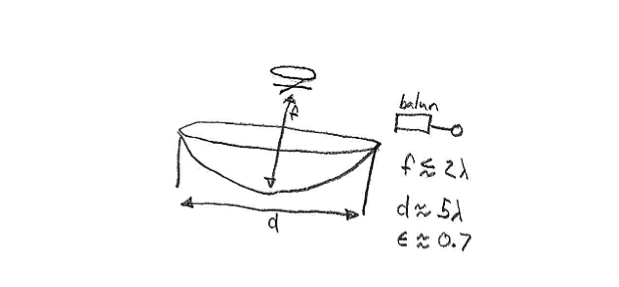
\includegraphics[width=3in]{dish_plots/eor_dish.png}
\caption{}
\label{fig:element_dish}
\end{figure}

This element concept is novel, but bears similarities to a drift-scan observing
mode explored on the GMRT, and to the cylinder dish concept being explored for
CHIME.  

In order for a parabolic (or cylindrical) dish to work for 21cm intensity
mapping, the focal length and dish diameter must be carefully controlled to
avoid reflections that enter at a significant delay, and thus modulate
foregrounds to corrupt scales at the corresponding $k_\parallel$.  Based on
recent work characterizing foregrounds, it seems reasonable to ask that a dish
not create more spectral structure than the shortest ($8\lambda\approx15$m)
baselines that have been shown to be well-behaved.  Beyond limiting the dish
diameter to 15m, this requirement restricts the focal length, since once of the
primary resonances in the dish will be the ``narcissistic waves'' that arise
between the primary and secondary reflector and/or the primary reflector and the
antenna feed.  These latter waves are a consequence of the necessarily imperfect
match of the feed electronics to the impedance of free space.

To mitigate narcissistic reflections, one typically adds an attenuator or
``splash cone'' directly below the feed.  If we posit that reflections must be
suppressed by $-60$dB at delays corresponding to the time it takes to travel
15m, and if we assume that reflections are attenuated by a factor $A$ for each
crossing of the attenuator placed below the feed, then the number of allowed
reflections, $R$, is given by
\begin{equation}
R={\rm floor}\left(\frac{-60{\rm dB}}{2A}\right).
\end{equation}
Thus, for a feed height (or focal length), $f$, we have
\begin{equation}
2Rf<15{\rm m}.
\end{equation}
For a moderate attenuation value of $A=-15$dB, we have $f<4$m.

\begin{figure}
\centering
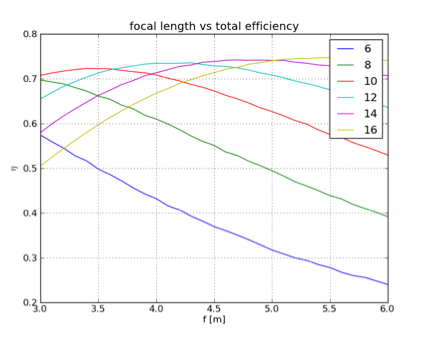
\includegraphics[width=4in]{dish_plots/focal_len_vs_eff.png}
\caption{Total efficiency as a function of focal length, for various diameters
of parabolic dishes (in meters).  Choosing a fiducial focal length of $f=3.5$m,
dish diameters of $10\le d\le 12$m yield efficiencies of $\eta\sim0.7$.}
\label{fig:focal_len_vs_eff}
\end{figure}

As shown in Figure \ref{fig:focal_len_vs_eff}, for a chosen focal length of
$f=3.5$m, dish diameters in the range of 10 to 12m yield efficiencies of
$\epsilon\approx0.7$.  Hence, the total effective collecting area of a dish that
has been tuned for 21cm intensity mapping at EoR frequencies is of order $80{\rm
m}^2$.  The corresponding effective beam area at 150 MHz 
(noting the issue described in \S\ref{sec:beam_area}) is approximately
\begin{equation}
\Omega^\prime\approx0.06\ {\rm sr}.
\end{equation}

In addition to the substantial collecting area that this design provides, the
relatively narrow field of view associated with a larger dish may go a long way
toward mitigating some of the polarization leakage problems that are just on the
horizon of being discovered with current designs.  However, without concrete
measurements, this is largely speculation.

NEED REVISION:
A diameter of $10$m corresponds to a most efficient focal length of $3.60$m instead of
$3.50$m, $4.5$m for $14$m diameter.

\subsection{The Knee}
The eor power spectrum has an upward slope for low $k$-modes which levels off
around $k$ = 0.15. It would be nice to work inside this $k$-mode to say
something interesting about eor. This poses a problem due to the fact that
without knowing the width of our foregrounds, we can't say for sure which
$k$-modes are corrupted. We also don't want to limit the size of our antenna too
much so as to decrease our sensitivity. 

The corresponding $k$-mode for a dish diameter of 10 $m$ is 0.016 and for a dish
diameter of 14 $m$ is 0.023 (see Equation \ref{eqn:k_horizon}). Hence, we have
some room for the foreground width's. But, the problem is that we do not know
precisely what they are. 

In addition to the width of the foreground and the maximum delay of the
baseline, narcissistic reflections add into our $k$ budget. For a 10 and 14
meter diameter dish we expect to have a maximum efficiency at a focal length of
3.5 and 4.5 $m$, respectively. Nominally, we would like these reflections to be
60dB down upon entering the feed. Postulating that each reflection reduces the
power by 15 dB, we need four reflections for the right signal to enter our feed.
This corresponds to a delay of 45.9 ($k$=0.023)  and 59.0 ($k$=0.030) $ns$ for
focal lengths of 3.5 and 4.5 meters, respectively. Therefore, our budget comes
out the $k_{10}$ = 0.039 and $k_{14}$ = 0.053.

As long as the width of the foregrounds are less than $\Delta k < 0.1$, we are
in good shape to working in the knee. 


\section{Construction}
See contruction_journal.tex

\end{document}
